\documentclass{article}
\usepackage[margin=0.5in,vmargin=0.5in]{geometry}
\usepackage{tikz}
\usepackage{graphicx}

%% neural network parameters
\newcommand\widthCirc{.5} % size of all circles
\newcommand\otdis{5} % distance between layers
\newcommand\nodeSep{2} % node seperation along y axis
\newcommand\inputNodes{4} % input node count
\newcommand\hiddenNodes{5} % hidden node count
\newcommand\outputNodes{2} % output node count
\newcommand\inputSRow{1} % vertical off-set of input layer
\newcommand\hiddenSRow{0} % vertical off-set of hidden layer
\newcommand\outputSRow{3} % vertical off-set of output layer
\newcommand\numLayers{3} % number of layers ommiting output layer


\newcommand\twohiddenNodes{5} % second hidden layer node count
\newcommand\twohiddenSRow{0} % vertical off-set of second hidden layer


\begin{document}

\begin{centering}

  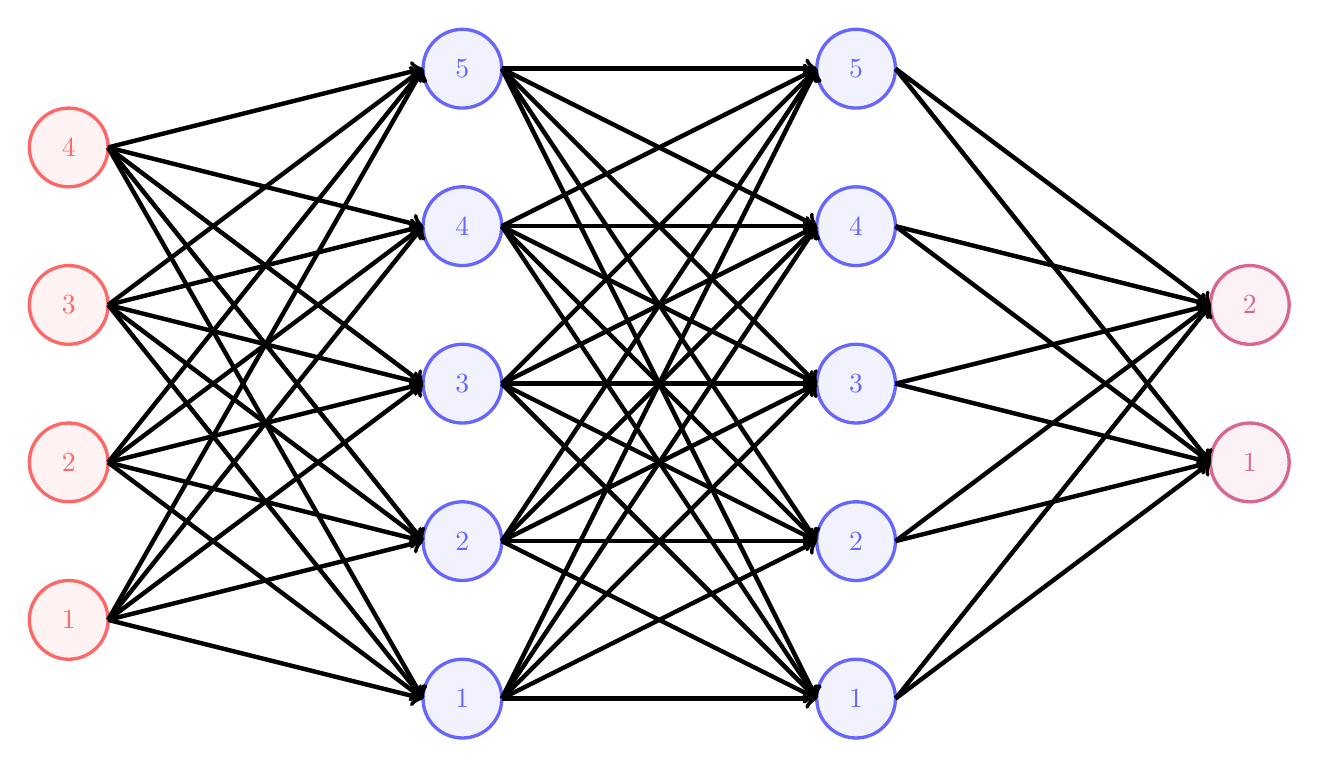
\begin{tikzpicture}
    \foreach \Rnumber in {1,...,\inputNodes}{
      \filldraw[color=red!60, fill=red!5, very thick](0,\inputSRow+\nodeSep*\Rnumber) circle (\widthCirc) node {$\Rnumber$};
    }
    
    \foreach \Rnumber in {1,...,\hiddenNodes}{
      \filldraw[color=blue!60, fill=blue!5, very thick](\numLayers*\otdis-2*\otdis,\hiddenSRow+\nodeSep*\Rnumber) circle (\widthCirc) node {$\Rnumber$};
    }

    \foreach \Rnumber in {1,...,\twohiddenNodes}{
      \filldraw[color=blue!60, fill=blue!5, very thick](\numLayers*\otdis-1*\otdis,\twohiddenSRow+\nodeSep*\Rnumber) circle (\widthCirc) node {$\Rnumber$};
    }
    
    \foreach \Rnumber in {1,...,\outputNodes}{
      \filldraw[color=purple!60, fill=purple!5, very thick](\numLayers*\otdis,\outputSRow+\nodeSep*\Rnumber) circle (\widthCirc) node {$\Rnumber$};
    }


    \foreach \Rnumber in {1,...,\inputNodes}{
      \foreach \Cnumber in {1,...,\hiddenNodes}{
        \draw[ultra thick, ->] (0+\widthCirc,\inputSRow+\nodeSep*\Rnumber) -- (\otdis-\widthCirc,\hiddenSRow+\nodeSep*\Cnumber) node {};
      }
    }


    \foreach \Rnumber in {1,...,\hiddenNodes}{
      \foreach \Cnumber in {1,...,\twohiddenNodes}{
        \draw[ultra thick, ->] (\numLayers*\otdis-2*\otdis+\widthCirc,\hiddenSRow+\nodeSep*\Rnumber) -- (\numLayers*\otdis-\otdis-\widthCirc,\twohiddenSRow+\nodeSep*\Cnumber) node {};
      }
    }

    \foreach \Rnumber in {1,...,\twohiddenNodes}{
      \foreach \Cnumber in {1,...,\outputNodes}{
        \draw[ultra thick, ->] (\numLayers*\otdis-\otdis+\widthCirc,\twohiddenSRow+\nodeSep*\Rnumber) -- (\numLayers*\otdis-\widthCirc,\outputSRow+\nodeSep*\Cnumber) node {};
      }
    }


  \end{tikzpicture}
\end{centering}

\end{document}
